\section{RISC-V Cores}

\subsection{Selection criteria}
The first step for developing the project is to select a suitable riscv implementation. Therefore, we defined the following guidelines for the decision:
\begin{itemize}
\item Multicore capable design.
\item Open or accessible design.
\item The resource usage of the core must fit the capabilities of our FPGA. In addition, we must take into account that we are aiming for a multicore target. Therefore, resource usage is critical.
\item Maximize the compatibility with our \gls{fpga}. Each \gls{fpga} has its own devices and peripherals such as memory, clock, and ports. Hence we should look for designs that are well integrated with our device to ease the deployment of the core into our \gls{fpga}.
\item As the project aims to boot something, we thought of finding a design that can boot Linux.
\end{itemize}

\subsection{Ariane}
Ariane is a 6 stage CPU initially developed at ETH Zurich. It fully supports I, A, M and C extensions which enable the core to boot Linux.

The standalone design cannot be multicore. However, Openpiton enables the design to be multicore. Openpiton\cite{openpiton} is an Open Source framework for building scalable architecture research prototypes from 1 to 500 million cores.

Figure \ref{fig:openpitonariane} shows the proposed architecture by OpenPiton designers. First, each Ariane core has its L1 cache and then an adapter for the OpenPiton cache. Next, a P-Mesh controller is attached to each core with an additional cache (L1.5), routing and a shared and distributed L2 cache with a directory-based coherence protocol. Then a 2D-mesh is formed with the tiles (P-mesh controller + Ariane core). 

\begin{figure}[h]
    \centering
    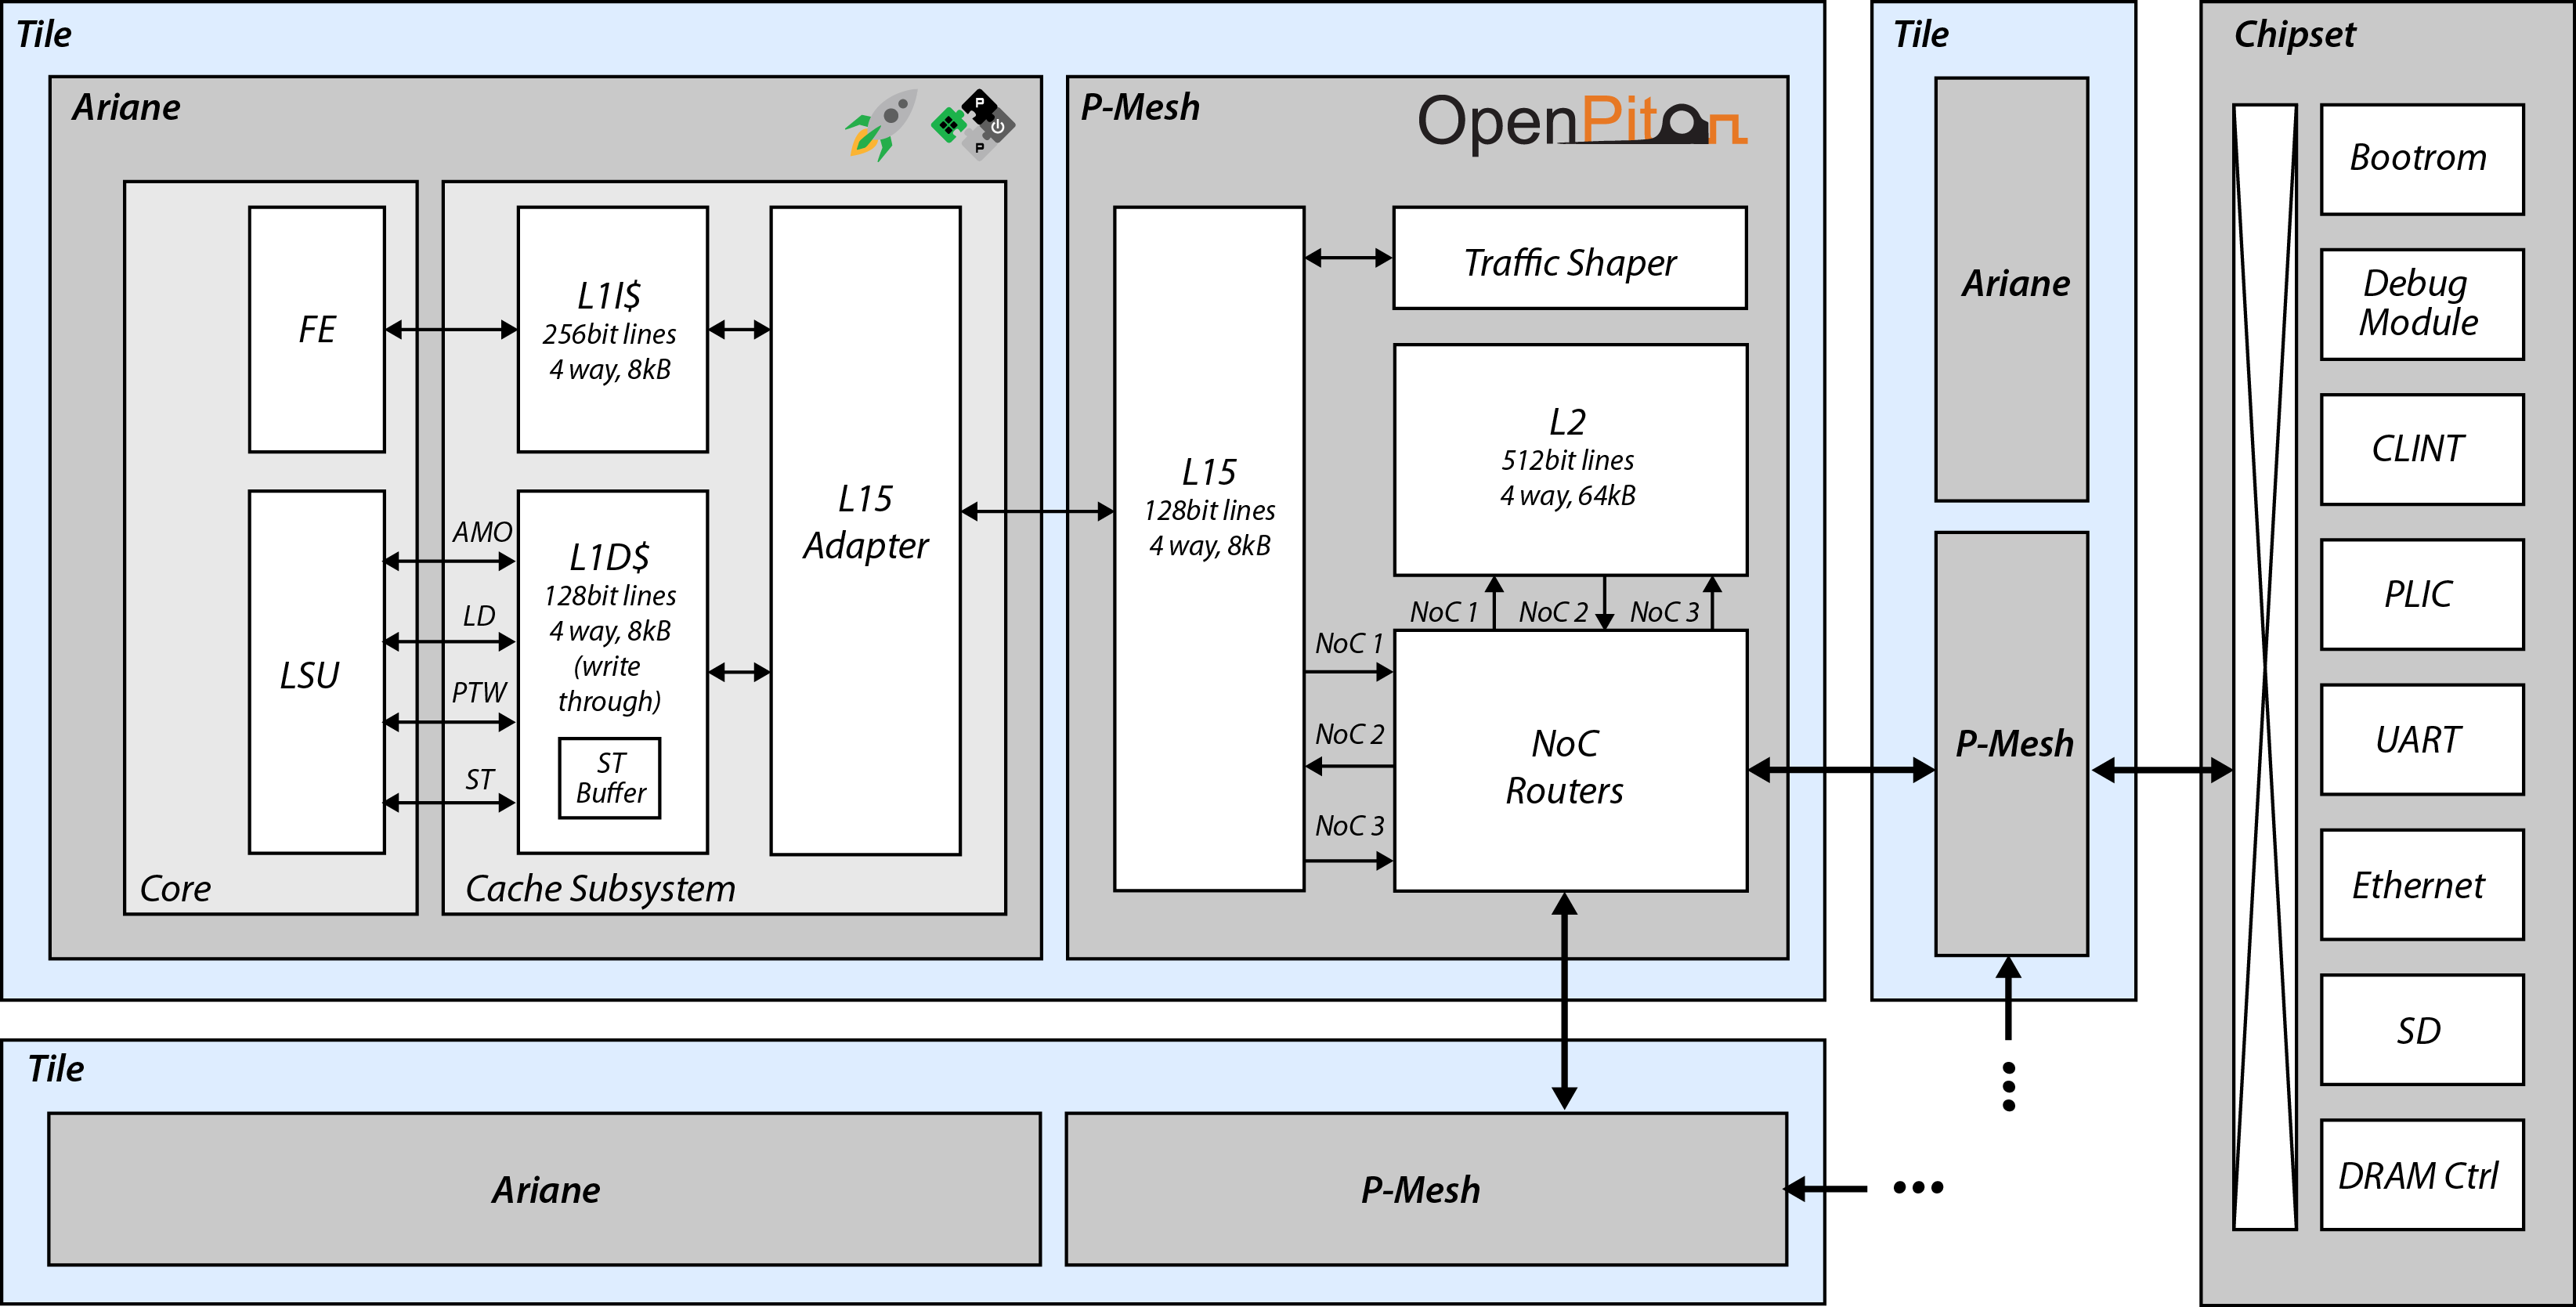
\includegraphics[width=0.9\textwidth]{img/openpiton_ariane_blockdiag.png}
    \caption{Openpiton and ariane block diagram.}
    \label{fig:openpitonariane}
\end{figure}

The main issue we encountered when trying to deploy the core was generating the bitstream. The design only officially supports the "Genesys2", "Nexys Video", and "VC707" boards. We tried to port and adapt it to our board, but we could not manage to do it. We decided to try another core because of the considerable complexity of the project and the knowledge needed to make the portability to our board possible.

\subsection{Rocketchip}
Rocketchip is a \gls{soc} generator designed at the University of Berkeley, California \cite{rocket}. From a configuration, it generates the full implementation, including multiple cores, caches and coherence protocol. It uses Chisel\footnote{\url{https://github.com/chipsalliance/chisel3}} as \gls{hdl}, a Scala-based language for \gls{asic} and \gls{fpga} logic designs. It implements the RISCV64G \gls{isa} variant. It is capable of booting Linux and allow different multicore configurations.

Figure \ref{fig:rocketstruct} shows \gls{soc} structure. The Rocketchip uses Rocket, BOOM or Zscale cores as a basic unit. Each core has its L1 data and instruction caches and a RoCC coprocessor. These units (Tiles) are interconnected using Tilelink, which interconnects the tiles with the level two cache. Tilelink is flexible and allows different cache coherence protocols. Finally, an AXI4 bridge connects the Tilelink module with the AXI4 crossbar, enabling the cores to access various devices and peripherals such as the \gls{dram}, IO devices.

\begin{figure}[h]
  \centering
  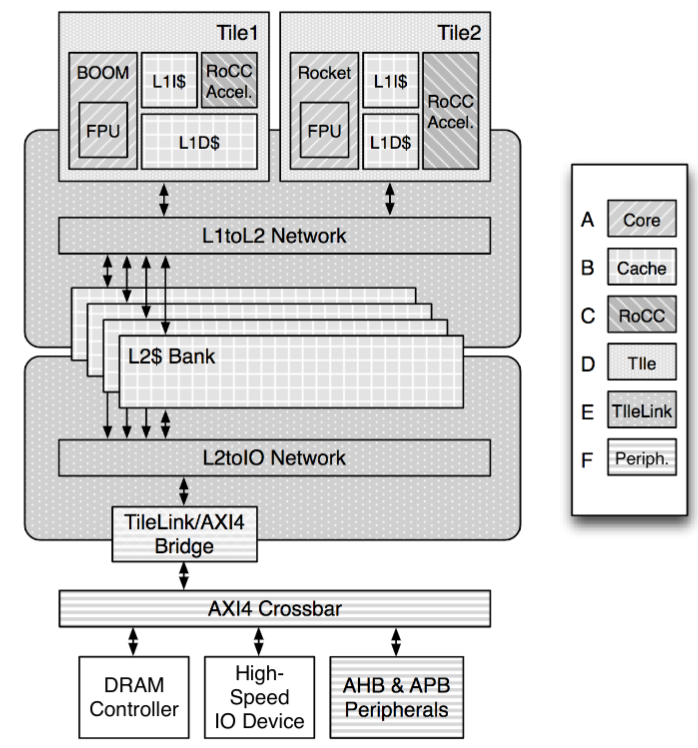
\includegraphics[width=0.6\textwidth]{images/rocket_structure.png}
  \caption{Rocketchip \gls{soc} structure}
  \label{fig:rocketstruct}
\end{figure}

When trying to deploy the Rocketchip \gls{soc}, we found out many difficulties. In particular, the lack of documentation, the Scala-based configuration and the resource usage made the deployment impossible.

\subsection{Darkriscv}
From the previous experience, we decided to take a different approach. We looked for a core that seems simple to deploy to our board and understand and then make the necessary modifications to accomplish project objectives.

Darkriscv\footnote{\url{https://github.com/darklife/darkriscv}} is a tiny and naive core that implements most of the RISCV32E and RISCV32I extensions. It uses few \gls{fpga} resources, and it has been tested on similar \gls{fpga} boards. The core is not designed to be multicore either to boot Linux. Therefore, we decided to rephrase the project objectives and defined new ones. First, to deploy Darkriscv into our \gls{fpga}, modify the design to be multicore capable, including a simple coherence system and boot simple programs to test the multicore design.

Its simplicity makes the design easy to understand, which enabled us to make the necessary modifications towards generating a bitstream for our \gls{fpga}.

Figure \ref{fig:bitstream_gen} illustrates the bitstream generation process. 
First, we create the Vivado project and import the source code files of Darkrsicv. Then we generate the constraints file, which maps between the hardware physical inputs and outputs to logical inputs and outputs for our code. In addition, we create the block design. Figure \ref{fig:block_design} shows the structure. We placed two blocks, a Xilinx Clock IP for our board and the Darksoc block, which contains the core. Then we connected the Xilinx clock to the Darksoc clock, the physical reset button to the core reset, the core LEDs to the board physical LEDs and the system clock to the Xilinx clocking IP.

\begin{figure}[h]
    \centering
    \begin{tikzpicture}[node distance=0.4cm]
      \node (prj) [stylepop] {Create Vivado project};
      \node (const) [stylepop, right=of prj ] {Design constraints file};
      \node (blk) [stylepop, right=of const] {Block design};
      \node (bit) [stylepop, right=of blk] {Generate bitstream};

      \draw [arrow] (prj) -- (const);
      \draw [arrow] (const) -- (blk);
      \draw [arrow] (blk) -- (bit);
    \end{tikzpicture}
    \caption{Bitstream generation process}
    \label{fig:bitstream_gen}
\end{figure}

\begin{figure}[h]
  \centering
  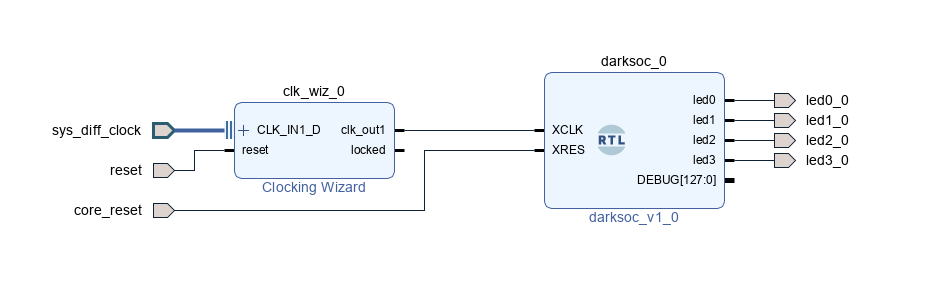
\includegraphics[width=0.8\textwidth]{../presentation/images/block-design.png}
  \caption{Darkriscv block design}
  \label{fig:block_design}
\end{figure}

Finally, once we have the block design, we are capable of synthesizing and generating the bitstream. 

\iffalse
[1] http://parallel.princeton.edu/openpiton/paper.html
[2] https://github.com/PrincetonUniversity/openpiton/blob/openpiton/docs/openpiton_ariane_blockdiag.png?raw=true
[3] https://www2.eecs.berkeley.edu/Pubs/TechRpts/2016/EECS-2016-17.html
[4] https://github.com/chipsalliance/chisel3
[5] Slides
[6] Slides

\fi